\chapter{实验与分析}

本章在Intel Core i5-1135G7平台上对前述攻击框架进行系统性的实验验证和量化评估。实验涵盖AES-128、AES-192和AES-256三种密钥长度变体，每种变体分别测试基准配置（无缓解措施）和四种缓解配置（低/中/高强度随机噪声注入、缓存刷新），每轮配置运行30次完整攻击以获得统计可靠的评估结果。实验内容分为三个层面：首先通过基准测试验证攻击框架的正确性和有效性，测量缓存命中/未命中的时间分布并校准分类阈值；其次对比不同缓解配置下的攻击成功率和泄露带宽，量化各防御措施的实际防护效果；最后深入分析泄露带宽与成功率之间的非线性关系、多阶段攻击的级联误差放大效应等关键现象。本章的实验数据将为第三章设计的攻击方法和缓解措施提供实证支撑，同时揭示Flush+Reload侧信道攻击在实际系统环境中的威胁程度和防御可行性。

\section{实验环境}

\subsection{硬件平台}

实验所用处理器为Intel Core i5-1135G7（Tiger Lake微架构），该处理器拥有4个物理核心、8个逻辑线程（支持超线程），基础频率2.40GHz，最大睿频4.20GHz。其缓存层次结构参数见表~\ref{tab:cpu_cache}。

\begin{table}[htbp]
    \centering
    \caption{实验平台处理器缓存参数。L1d和L2为各核私有，L3为所有核心共享。缓存行大小为64字节}
    \label{tab:cpu_cache}
    \begin{tabular}{ccccc}
        \toprule
        缓存层级 & 容量 & 相联度 & 写策略 & 共享范围 \\
        \midrule
        L1d & 48KB & 12路 & 写回 & 单核私有 \\
        L2 & 1.25MB & 20路 & 写回 & 单核私有 \\
        L3 & 8MB & 12路 & 写回 & 全核共享 \\
        \bottomrule
    \end{tabular}
\end{table}

L3为全核共享，即使攻击者和受害者运行于不同的逻辑核心上，攻击者也能用clflush指令将目标缓存行从整个缓存层次中驱逐，然后通过reload的延迟判断受害者是否再次访问了该行。

64字节的缓存行大小意味着T表每个表项（256个4字节uint32\_t元素，恰好占1KB）跨越16个缓存行。攻击者可以逐行监控，获取细粒度的访问模式。

T表总大小（4$\times$1KB=4KB）远小于L3容量，不会因缓存容量不足而被意外驱逐。这为攻击提供了稳定的缓存驻留条件。

\subsection{软件环境}

操作系统为Ubuntu 20.04 LTS，Linux内核版本5.15.0。编译器采用GCC 9.4.0，编译选项为\texttt{-O0 -march=native}。\texttt{-O0}不开启优化，保证T表访问不被编译器优化掉，这对Flush+Reload攻击至关重要。\texttt{-march=native}使编译器针对Tiger Lake微架构生成特定指令序列，包括对\texttt{rdtsc}、\texttt{clflush}等指令的支持。

内核配置方面，实验中关闭了地址空间布局随机化（ASLR），以排除ASLR对共享库内存映射的影响。同时禁用了CPU频率动态调节（通过将scaling\_governor设为performance模式），确保CPU始终运行在标称频率，避免因频率波动导致的时间测量偏差。此外，实验保留了超线程功能，Attacker和Victim均通过sched\_setaffinity绑定到同一逻辑核心（CPU~0），两个进程在该核心上交替执行，共享同一套L1d/L2缓存，确保缓存状态的变化直接反映受害者的访问行为。

\subsection{实验参数}

实验参数设置如下：AES-128、AES-192、AES-256的样本量分别为5000、9000、15000，每种配置运行30轮。

测试了5种缓解配置：Baseline（无缓解措施）、Noise-Low（30\%访问概率）、Noise-Medium（40\%访问概率）、Noise-High（50\%访问概率）、Cache-Flush（加密后刷新T表监控缓存行）。

\section{基准测试结果}

\subsection{攻击成功率}

AES-128/192/256各运行30轮完整成功率测试，在基准测试下（无缓解措施），三种变体的成功率均为100\%（30/30）。在受控实验环境中，缓存命中与未命中时间表现出显著的、无重叠的双峰分布，这使得分类器能以极低的误判率工作。当样本量足以满足排除法所需的统计置信度时，密钥恢复成功率达到100\%是符合理论预期的。

实验样本量（分别为5000、9000、15000次加密）远超理论最低要求。对于AES-128的单字节攻击，由$89/p_{miss}$估算的理论最低样本量约为1171次，而实际需要恢复16个字节且保证联合置信度，所需样本量更高。实验采用的5000个样本为单字节恢复提供了充足的统计冗余，确保了高成功率。对于AES-192和AES-256的两阶段攻击，更大的样本量（9000和15000）同样提供了充足的统计冗余，使得基准成功率达到100\%。

\subsection{缓存时间分布与阈值校准}

缓存命中/未命中的时间分布统计见表~\ref{tab:cache_timing}。

\begin{table}[htbp]
    \centering
    \caption{缓存访问时间分布统计（校准阶段测量）。命中时间中位数（118周期）与未命中时间中位数（347周期）相差约229周期，P5--P95范围内无重叠，说明基于中位数的阈值设置能可靠地区分命中和未命中这两种状态}
    \label{tab:cache_timing}
    \begin{tabular}{ccc}
        \toprule
        统计量 & 命中时间（周期） & 未命中时间（周期） \\
        \midrule
        中位数 & 118.0 & 347.0 \\
        第一四分位数（Q1） & 116.0 & 344.0 \\
        第三四分位数（Q3） & 120.0 & 362.0 \\
        第5百分位数（P5） & 108.0 & 333.0 \\
        第95百分位数（P95） & 132.0 & 508.0 \\
        \bottomrule
    \end{tabular}
\end{table}

阈值校准过程如下：在攻击开始前，攻击者对目标缓存行执行10000次clflush and reload测量，记录每次reload的CPU周期数。将测量结果按升序排列，分别取命中时间和未命中时间的中位数$M_{\text{hit}}$和$M_{\text{miss}}$，取两者中点作为分类阈值$T$：

\begin{equation}
T = \frac{M_{\text{hit}} + M_{\text{miss}}}{2}
\end{equation}

在本实验中，$T = (118 + 347) / 2 = 233$周期。reload时间低于$T$判定为命中，高于$T$判定为未命中。

\section{缓解措施对比测试}

\subsection{噪声缓解措施机制}

噪声缓解的思路是：加密之后按一定概率干扰T表缓存行，打乱攻击者看到的缓存状态。Victim完成AES加密后，以预设概率对4个T表的第0号缓存行执行内存读取操作（mov指令），将该缓存行重新加载到CPU缓存中。这样，即使Victim加密时未访问某个T表的第0缓存行（攻击者本应观察到cache miss），噪声读取也会让攻击者看到cache hit，从而引入假阳性，降低排除法密钥恢复的准确性。需要指出，本实验的噪声注入仅针对每张T表的第0号缓存行，即与攻击者监控目标相同的缓存行。这是一种针对性的噪声策略：由于攻击者只监控第0缓存行，噪声也只需干扰该行的观测即可。

\subsection{AES-128缓解措施对比}

AES-128的结果见表~\ref{tab:aes128_mitigation}。

\begin{table}[htbp]
    \centering
    \caption{AES-128缓解措施对比测试结果（30轮，样本量5000）。噪声越强，成功率越低，泄露带宽也越低。Cache-Flush下泄露带宽归零}
    \label{tab:aes128_mitigation}
    \begin{tabular}{cccc}
        \toprule
        配置 & 成功率 & 泄露带宽(bps) \\
        \midrule
        Baseline & 100\% & 60759 \\
        Noise-Low (30\%) & 100\% & 26079 \\
        Noise-Med (40\%) & 90\% & 21873 \\
        Noise-High (50\%) & 46\% & 12467 \\
        Cache-Flush & 0\% & 0 \\
        \bottomrule
    \end{tabular}
\end{table}

AES-128的攻击仅需恢复16字节密钥，采用单阶段攻击即可完成。

在Noise-Low（30\%）配置下，AES-128的成功率仍为100\%，说明低噪声概率对单阶段攻击影响有限；在Noise-Medium（40\%）配置下，成功率降至90\%；在Noise-High（50\%）配置下，成功率降至46\%，50\%的噪声概率对单阶段攻击产生显著影响。

关于泄露带宽：AES-128在Noise-High下泄露带宽约12kbps，从基准的约61kbps降至约12kbps，降幅达79\%。泄露带宽随噪声增强而下降，成功率也相应下降，说明噪声缓解对单阶段攻击有明显效果。

\subsection{AES-192缓解措施对比}

AES-192的结果见表~\ref{tab:aes192_mitigation}。

\begin{table}[htbp]
    \centering
    \caption{AES-192缓解措施对比测试结果（30轮，样本量9000）。AES-192要走两阶段攻击，对噪声更敏感}
    \label{tab:aes192_mitigation}
    \begin{tabular}{cccc}
        \toprule
        配置 & 成功率 & 泄露带宽(bps) \\
        \midrule
        Baseline & 100\% & 34678 \\
        Noise-Low (30\%) & 93\% & 18080 \\
        Noise-Med (40\%) & 66\% & 12433 \\
        Noise-High (50\%) & 36\% & 9174 \\
        Cache-Flush & 0\% & 0 \\
        \bottomrule
    \end{tabular}
\end{table}

AES-192的密钥长度为24字节，攻击分两阶段：第一阶段恢复最后一轮子密钥$K_{12}$（16字节），第二阶段恢复倒数第二轮子密钥$K_{11}$（16字节），两者结合通过密钥扩展逆运算恢复原始24字节密钥。两阶段攻击对噪声更敏感，因为第二阶段的正确性依赖第一阶段的结果。第一阶段恢复的$K_{12}$一旦有任意字节出错，第二阶段的等效解密计算就会全部错误，导致$K_{11}$恢复失败。

两阶段攻击的整体成功率是两个阶段成功率的乘积，噪声对每个阶段的削弱效应会级联放大。

对比AES-128和AES-192在相同噪声配置下的表现：在Noise-Low（30\%）下，AES-192成功率降至93\%，而AES-128仍为100\%，两阶段攻击级联效应开始显现；在Noise-Medium（40\%）下，AES-192成功率为66\%，而AES-128为90\%；在Noise-High（50\%）下，AES-192成功率降至36\%，远低于AES-128的46\%。这个现象说明AES-192的两阶段攻击结构在噪声下级联效应显著，高噪声下成功率下降幅度明显大于单阶段攻击。

\subsection{AES-256缓解措施对比}

AES-256的结果见表~\ref{tab:aes256_mitigation}。

\begin{table}[htbp]
    \centering
    \caption{AES-256缓解措施对比测试结果（30轮，样本量15000）。AES-256对噪声最敏感}
    \label{tab:aes256_mitigation}
    \begin{tabular}{cccc}
        \toprule
        配置 & 成功率 & 泄露带宽(bps) \\
        \midrule
        Baseline & 100\% & 23584 \\
        Noise-Low (30\%) & 66\% & 10758 \\
        Noise-Med (40\%) & 40\% & 8329 \\
        Noise-High (50\%) & 20\% & 6032 \\
        Cache-Flush & 0\% & 0 \\
        \bottomrule
    \end{tabular}
\end{table}

AES-256对噪声最为敏感。在Baseline配置下成功率为100\%；在Noise-Low（30\%）配置下成功率降至66\%；在Noise-Medium（40\%）配置下成功率降至40\%；在Noise-High（50\%）下成功率降至20\%。

一个自然的问题是：AES-256和AES-192的攻击结构完全相同——都是两阶段攻击，每个阶段恢复16字节轮密钥——为什么AES-256在各噪声配置下的成功率均显著低于AES-192？答案不在于阶段数的差异，而在于每阶段能获取的有效信息量不同。AES-256因加密轮数更多，导致攻击中"有效排除样本"更少，单字节恢复的可靠性更低；而两阶段攻击的级联放大效应将这一微小差异急剧放大，最终导致成功率显著下降。下面从三个层面展开分析。

（1）核心差异：每阶段的有效信息量。AES-192和AES-256的攻击结构相同：第一阶段恢复最后一轮子密钥（AES-192恢复$K_{12}$，AES-256恢复$K_{14}$），第二阶段恢复倒数第二轮子密钥（AES-192恢复$K_{11}$，AES-256恢复$K_{13}$），然后通过密钥扩展逆运算得到原始密钥。关键区别在于加密轮数不同导致有效排除样本数量不同。AES-192有12轮加密，每个T表被访问48次；AES-256有14轮加密，每个T表被访问56次。攻击依赖的是"某个缓存行在整次加密中从未被访问"这一事件，其发生概率为：
\begin{equation}
p_{miss} = \left(\frac{15}{16}\right)^{\text{访问次数}}
\end{equation}
AES-192的$p_{miss} \approx 0.045$，AES-256的$p_{miss} \approx 0.027$。AES-256的有效排除样本数量天生比AES-192少约40\%，单字节恢复的可靠性更低。

（2）级联放大效应：微小差异被乘积急剧放大。两阶段攻击的整体成功率是阶段一和阶段二成功率的乘积，而阶段二的正确性完全依赖阶段一的结果——阶段一恢复的轮密钥一旦有任意字节出错，阶段二的等效解密计算就会全部错误。设阶段一恢复16字节密钥的成功概率为$P_1 = p_{byte}^{16}$，阶段二在阶段一正确条件下的成功概率为$P_{2|1} \approx p_{byte}^{16}$，则整体成功概率近似为：
\begin{equation}
P_{total} = P_1 \times P_{2|1} \approx p_{byte}^{32}
\end{equation}
若AES-192的$p_{byte} = 0.99$，则$0.99^{32} \approx 0.72$；若AES-256的$p_{byte} = 0.97$，则$0.97^{32} \approx 0.38$。单字节可靠性仅差2个百分点，经过32次乘积后成功率几乎减半。实验数据也证实了这一点：在Noise-Low下AES-192成功率为93\%而AES-256为66\%，在Noise-Medium下分别为66\%和40\%，在Noise-High下分别为36\%和20\%，差距随噪声增强而持续扩大。

（3）噪声对AES-256打击更重。噪声注入进一步压缩有效未命中率：
\begin{equation}
p_{miss}' = p_{miss} \times (1 - p_{noise})
\end{equation}
以Noise-High（$p_{noise} = 0.5$）为例，AES-192的有效未命中率从0.045降至0.0225，AES-256从0.027降至0.0135。AES-256的底层信息本来就少，再被噪声压缩，有效信息更加稀缺。而两阶段攻击中阶段二的输入完全依赖阶段一的输出——阶段一错一个字节，阶段二全错——这就是级联失败。

综合以上三个层面，AES-256比AES-192更难攻破的根本原因可以概括为：两者攻击阶段数相同，但AES-256因加密轮数更多（14轮 vs 12轮）导致$p_{miss}$更低（0.027 vs 0.045），每阶段有效信息量少约40\%，单字节恢复的可靠性更低；而两阶段攻击需要同时恢复32个字节的轮密钥，32次乘积的级联放大效应将微小的单字节可靠性差异急剧放大——单字节成功率仅差2个百分点，整体成功率几乎减半；噪声注入进一步压缩本已稀缺的有效信息，使级联失败更加严重。

再看样本量与成功率的关系。三种AES变体分别使用5000、9000、15000次样本，但在噪声环境下AES-256仍然最难攻破。这说明：对于多阶段攻击，仅依靠增加样本量无法有效对抗噪声。每个阶段的错误会向后续阶段传播，更多样本仅能提升单个阶段的置信度，无法解决级联失败这一结构性问题。

\subsection{三种AES缓解措施对比}

三种AES在各缓解配置下的成功率，见图~\ref{fig:success_rate_comparison}。

\begin{figure}[htbp]
    \centering
    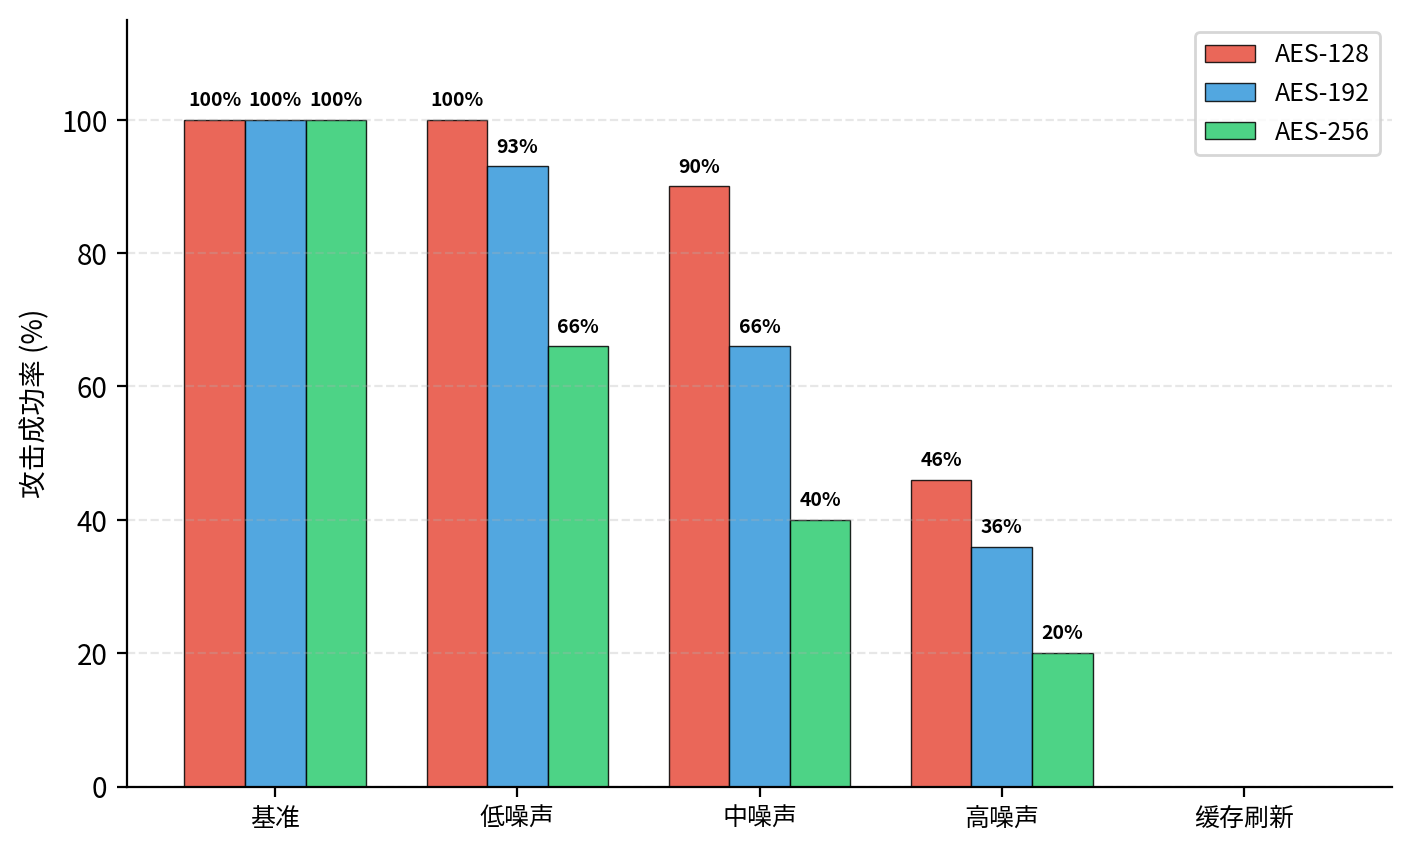
\includegraphics[width=0.9\textwidth]{figures/thesis_success_rate.png}
    \caption{三种AES在不同缓解措施下的攻击成功率对比（30轮）。Baseline时三种AES成功率均为100\%。随着噪声提高，成功率会降低，密钥越长降低越快。Cache-Flush使成功率降至零}
    \label{fig:success_rate_comparison}
\end{figure}

图~\ref{fig:success_rate_comparison}直观地表明：三种AES变体的成功率随噪声强度增加而下降的速率差异显著。AES-128在Noise-Low下成功率仍为100\%，Noise-Medium下降至90\%，Noise-High下降至46\%，单阶段攻击对噪声相对鲁棒；AES-192在Noise-Low下为93\%，Noise-Medium下降至66\%，Noise-High下降至36\%，两阶段攻击级联效应显著；AES-256在Noise-Low下为66\%，Noise-Medium下为40\%，Noise-High下为20\%，级联效应使噪声的影响被急剧放大。差异的根源在于：AES-256加密轮数更多导致$p_{miss}$更低、每阶段有效信息量更少，而两阶段攻击的32字节乘积级联将微小的单字节可靠性差异急剧放大。

进一步分析另一现象：AES-256在Noise-Medium下泄露带宽约8kbps，成功率40\%；AES-192在Noise-Medium下泄露带宽约12kbps，成功率66\%。虽然AES-256的泄露带宽更低，但其成功率下降更剧烈。这说明噪声缓解并未完全消除侧信道的信息泄露，仅将泄露量降至攻击者难以有效利用的水平。从防御角度而言，这意味着仅依靠噪声可能不足。如果攻击者采用了更先进的信号处理或统计推断技术，仍可能从残余泄露中提取密钥。相比之下，Cache-Flush使泄露带宽降为零，防护更为彻底。

\section{量化指标分析}

\subsection{泄露带宽分析}

泄露带宽定义为单位时间内从缓存侧信道泄露的信息量（单位：bit/s），计算公式为：

\begin{equation}
BW = 4 \cdot MI_{binary} \cdot f_{sample}
\end{equation}

其中$MI_{binary}$为单次缓存行观测的互信息（bit/观测），$f_{sample}$为采样频率（次/秒），系数4对应每次采样对4个缓存行各进行一次独立观测。

泄露带宽的下降幅度与AES变体和噪声强度直接相关。以基准泄露带宽为参照：

\begin{itemize}
    \item AES-128：Noise-Low下降57\%（60759$\to$26079bps），Noise-Medium下降64\%（$\to$21873bps），Noise-High下降79\%（$\to$12467bps）
    \item AES-192：Noise-Low下降48\%（34678$\to$18080bps），Noise-Medium下降64\%（$\to$12433bps），Noise-High下降73\%（$\to$9174bps）
    \item AES-256：Noise-Low下降54\%（23584$\to$10758bps），Noise-Medium下降65\%（$\to$8329bps），Noise-High下降74\%（$\to$6032bps）
\end{itemize}

一个有趣的发现是：泄露带宽的下降幅度在三种AES变体间总体接近，但在低噪声级别下仍存在一定差异。Noise-Low下三种变体的降幅分别为57\%、48\%、54\%，极差为9个百分点；而Noise-Medium和Noise-High下极差缩小至1--6个百分点。相比之下，成功率的下降差异在所有噪声级别下均十分显著。例如，Noise-High下三种变体的泄露带宽降幅都在73\%--79\%之间，但AES-128成功率为46\%，AES-192为36\%，AES-256仅为20\%。这再次说明成功率下降的主因是AES-256每阶段有效信息量更少加之32字节乘积级联放大，而非单纯的泄露量减少。

Cache-Flush下攻击者无法获得任何信息，泄露带宽归零。图~\ref{fig:leakage_bw}展示了泄露带宽的变化趋势。

\begin{figure}[htbp]
    \centering
    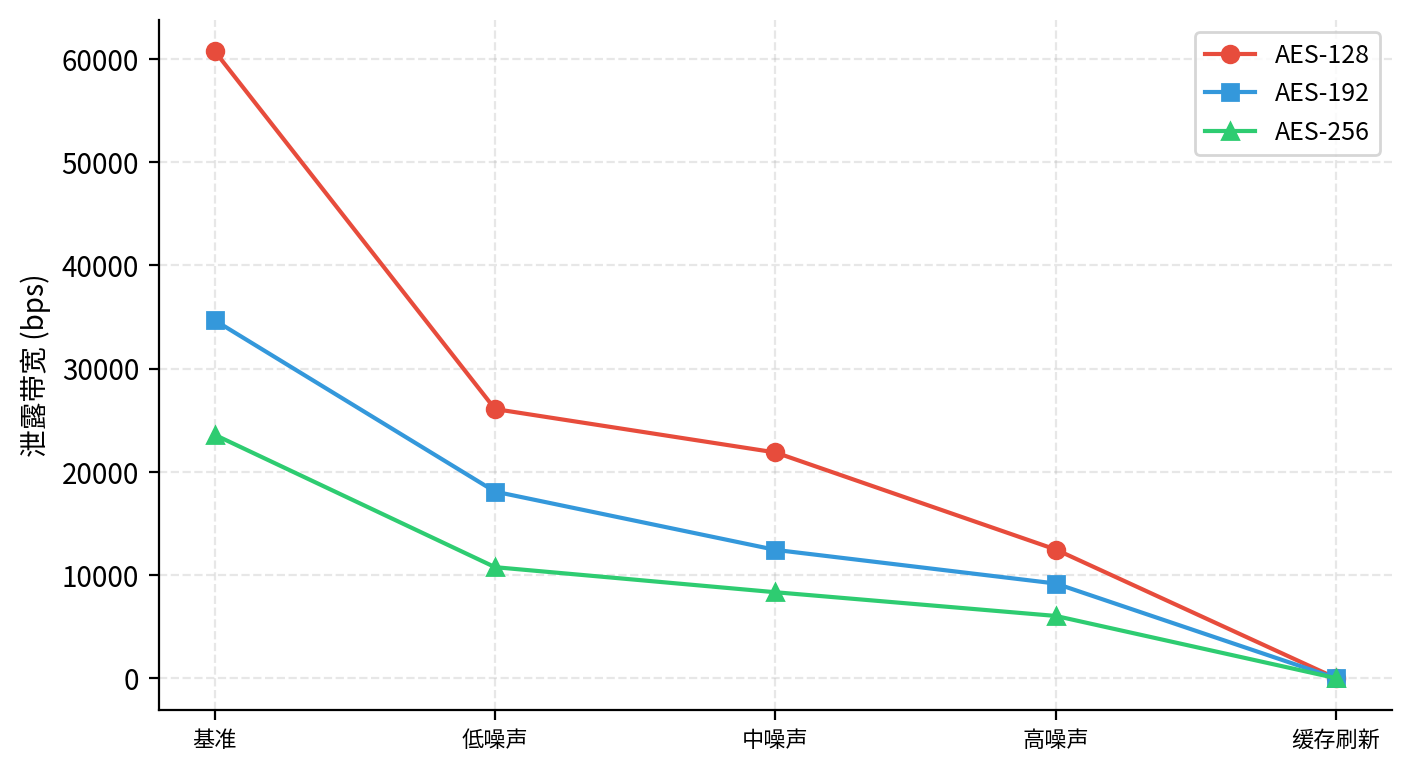
\includegraphics[width=0.9\textwidth]{figures/thesis_leakage_bw.png}
    \caption{三种AES在不同缓解措施下的泄露带宽（30轮）。Baseline：AES-128约61kbps，AES-192约35kbps，AES-256约24kbps。噪声越强，泄露带宽越低。Cache-Flush下即为零}
    \label{fig:leakage_bw}
\end{figure}

\subsection{泄露带宽与攻击成功率的关系}

泄露带宽与攻击成功率之间存在非线性关系。AES-128在Noise-High下泄露带宽约12kbps，成功率46\%；AES-256在Noise-High下泄露带宽约6kbps，成功率仅20\%。两者泄露带宽相差较大，但成功率差异更为显著。这说明对于AES-256，即使泄露量仍然较大，其更低的$p_{miss}$导致单字节可靠性更低，经过32字节乘积级联放大后成功率急剧下降。

\section{本章小结}

本章在Intel Core i5-1135G7平台上，对AES-128/192/256三种变体分别测试了基准配置和四种缓解配置，每种运行30轮。结论如下。

默认情况下三种AES变体成功率均为100\%。随着噪声强度的增加成功率呈下降趋势：AES-128在Noise-Low下为100\%，Noise-Medium下为90\%，Noise-High下为46\%，单阶段攻击对噪声相对鲁棒；AES-192在Noise-Low下为93\%，Noise-Medium下为66\%，Noise-High下为36\%，两阶段攻击级联效应显著；AES-256在Noise-Low下为66\%，Noise-Medium下为40\%，Noise-High下为20\%。AES-256与AES-192的攻击阶段数相同，但AES-256更难攻破的根本原因在于：14轮加密使$p_{miss}$更低（0.027 vs 0.045），每阶段有效信息量少约40\%，单字节恢复可靠性更低；而两阶段攻击需要同时恢复32个字节的轮密钥，级联放大效应将微小的单字节可靠性差异急剧放大；噪声注入进一步压缩本已稀缺的有效信息，使级联失败更加严重。缓存刷新是确定性防御，使成功率与泄露带宽均降至零，防护最为彻底。

泄露带宽随噪声增强而下降，缓存刷新下归零。但泄露带宽与成功率之间并非线性关系：AES-128在Noise-High下泄露带宽约12kbps，成功率46\%；AES-256在Noise-High下泄露带宽约6kbps，成功率仅20\%。两者泄露带宽相差较大，但成功率差异更为显著，AES-256更低的$p_{miss}$经32字节乘积级联放大后导致成功率急剧下降。
